\section{Mô hình Thị giác SOTA 2024–2025: EVA, ConvNeXt-V2, InternImage, FocalNet}
\label{sec:sota_vision_models_2024_2025}

\subsection{Tổng quan: Kỷ nguyên ''Hậu ViT''}
\label{subsec:post_vit_era_overview}
Sự ra đời của Vision Transformer (ViT) đã châm ngòi cho một cuộc chạy đua kiến trúc sôi nổi. Nếu giai đoạn 2020-2022 là thời kỳ của những khám phá và cải tiến nền tảng (như Swin Transformer, DeiT), thì giai đoạn 2023-2025 đánh dấu sự trưởng thành của kỷ nguyên "hậu ViT". Các mô hình trong giai đoạn này không chỉ đơn thuần là những biến thể của Transformer, mà là sự kết hợp tinh hoa từ nhiều trường phái, tập trung vào ba mục tiêu chính:
\begin{enumerate}
	\item \textbf{Khả năng Mở rộng (Scalability):} Làm thế nào để huấn luyện các mô hình ngày càng lớn hơn, trên các bộ dữ liệu quy mô web, một cách hiệu quả?
	\item \textbf{Tính Tổng quát (Generality):} Làm thế nào để xây dựng một \textbf{xương sống thị giác thống nhất (unified vision backbone)} duy nhất, có thể hoạt động xuất sắc trên nhiều tác vụ khác nhau (phân loại, phát hiện, phân đoạn) mà không cần tinh chỉnh quá nhiều?
	\item \textbf{Hiệu quả (Efficiency):} Làm thế nào để đạt được hiệu năng cao mà vẫn duy trì chi phí tính toán và bộ nhớ ở mức hợp lý?
\end{enumerate}
Phần này sẽ phân tích bốn trong số những họ kiến trúc tiêu biểu, dẫn đầu giai đoạn này, định hình nên tương lai của các mô hình thị giác: EVA, ConvNeXt-V2, InternImage, và FocalNet.

\subsection{EVA: Sức mạnh của Quy mô và Học Tự Giám Sát}
\label{subsec:eva_model}

\textbf{EVA (Exploring the Limits of Visual Representation Learning at Scale)} \cite{Fang2023} là dòng mô hình thị giác nền tảng (vision foundation models) do Microsoft Research phát triển, minh họa rõ triết lý “\textit{Scaling Laws}” – khi quy mô dữ liệu, mô hình và thời gian huấn luyện đủ lớn, hiệu năng sẽ tiếp tục tăng một cách có hệ thống.

\subsubsection{Động cơ và Triết lý}
Các mô hình Vision Transformer trước đó như ViT và MAE đã chứng minh khả năng học biểu diễn mạnh, nhưng vẫn bị giới hạn bởi:
\begin{itemize}
	\item Quy mô dữ liệu huấn luyện chưa đủ lớn, thường dừng lại ở mức ImageNet-1K (1.2M ảnh) hoặc JFT-300M.
	\item Thiếu sự kết nối giữa không gian thị giác và ngữ nghĩa (ngôn ngữ).
	\item Quá trình pre-training thường đắt đỏ, khó mở rộng, và chưa tối ưu cho downstream tasks.
\end{itemize}

EVA được thiết kế để vượt qua các rào cản này bằng cách kết hợp:
\begin{enumerate}
	\item Quy mô dữ liệu ở mức web-scale (tỷ ảnh).
	\item Học tự giám sát thông qua Masked Image Modeling (MIM).
	\item Căn chỉnh ngôn ngữ–hình ảnh thông qua học tương phản (contrastive fine-tuning).
\end{enumerate}

Triết lý của EVA có thể tóm gọn như sau:
\begin{center}
	\textit{"Scale up everything — data, model, and training — with self-supervised objectives that encourage semantic understanding."}
\end{center}

---

\subsubsection{Cơ chế Học Tự Giám Sát Hai Giai Đoạn}
\label{subsubsec:eva_self_supervised}

\textbf{1. Giai đoạn 1 – Masked Image Modeling (EVA-MIM):}  
Tương tự MAE \cite{He2022}, EVA học cách tái tạo lại các patch ảnh bị che khuất. Tuy nhiên, EVA nâng cấp quy mô và cơ chế huấn luyện:
\begin{itemize}
	\item Sử dụng các bộ dữ liệu mở quy mô web như \textbf{LAION-2B} và \textbf{COYO-700M}, tổng cộng hàng tỷ hình ảnh.  
	\item Thay vì tái tạo ảnh pixel-wise, EVA học biểu diễn trừu tượng trong không gian đặc trưng (feature reconstruction), giúp tập trung vào ngữ nghĩa thay vì chi tiết thấp.
	\item Mô hình hóa trên các biến thể ViT-L/ViT-H (Base/Large/Huge) với hàng tỷ tham số, sử dụng kỹ thuật huấn luyện song song và mixed precision.
\end{itemize}

\textbf{2. Giai đoạn 2 – Fine-tuning Tương phản Ngôn ngữ–Hình ảnh (EVA-CLIP):}  
Sau khi pre-train bằng MIM, EVA được tinh chỉnh bằng học tương phản đa phương thức:
\[
\mathcal{L}_{CLIP} = -\frac{1}{N}\sum_i \log \frac{\exp(\text{sim}(v_i, t_i)/\tau)}{\sum_j \exp(\text{sim}(v_i, t_j)/\tau)}
\]
trong đó $v_i$ và $t_i$ lần lượt là vector đặc trưng của ảnh và văn bản, $\text{sim}(\cdot)$ là cosine similarity, $\tau$ là hệ số nhiệt độ.  
Cách tiếp cận này tương tự CLIP \cite{Radford2021}, nhưng EVA tận dụng \textbf{embedding từ giai đoạn MIM} nên có biểu diễn thị giác sâu và tổng quát hơn.

Kết quả là mô hình EVA-CLIP vừa hiểu ngữ cảnh ngôn ngữ, vừa có khả năng biểu diễn thị giác mạnh mẽ, trở thành nền tảng cho nhiều nhiệm vụ downstream khác nhau.

---

\subsubsection{Kết quả và Hiệu năng}
\label{subsubsec:eva_results}

EVA và EVA-CLIP đạt hiệu năng kỷ lục trên hàng loạt benchmark:

\begin{itemize}
	\item \textbf{ImageNet-1K:} EVA-L đạt 89.7\% top-1 accuracy, vượt DINOv2 và MAE cùng quy mô.  
	\item \textbf{COCO Object Detection:} tăng +2.1 mAP so với Swin-L.  
	\item \textbf{ADE20K Semantic Segmentation:} mIoU đạt 57.4, cao nhất thời điểm 2023.
	\item \textbf{Zero-shot Transfer:} EVA-CLIP outperform CLIP và ALIGN trên nhiều tập dữ liệu downstream (Food101, OxfordPets, CIFAR-100, SUN397…).
\end{itemize}

Quan trọng hơn, EVA chứng minh rằng:
\begin{enumerate}
	\item Việc mở rộng quy mô và dùng tự giám sát (MIM + contrastive) có thể tạo ra \textbf{biểu diễn tổng quát hơn} so với học có giám sát truyền thống.
	\item ViT khi được huấn luyện ở quy mô web có thể trở thành \textbf{foundation model} cho toàn bộ miền thị giác, tương tự như cách GPT trở thành foundation model cho ngôn ngữ.
\end{enumerate}

---

\subsubsection{Tầm Ảnh hưởng và Vai trò trong Hệ sinh thái Foundation Models}
\label{subsubsec:eva_impact}

EVA đặt nền móng cho một thế hệ mới của mô hình thị giác, nơi:
\begin{itemize}
	\item Học \textbf{tự giám sát} thay thế hoàn toàn học có giám sát.  
	\item Mô hình được huấn luyện trên \textbf{dữ liệu mở quy mô web}, thay vì các tập dữ liệu đóng.  
	\item Biểu diễn thị giác trở thành \textbf{khối nền tảng đa nhiệm} – có thể dùng cho detection, segmentation, captioning, retrieval, và cả multimodal LLM.
\end{itemize}

Các mô hình sau này như \textbf{DINOv2 (Meta, 2023)}, \textbf{InternVL (Shanghai AI Lab, 2024)}, hay \textbf{Florence-2 (Microsoft, 2024)} đều chịu ảnh hưởng sâu sắc từ EVA — tiếp tục triết lý "scale everything" và củng cố vai trò của ViT như nền tảng của các hệ thống thị giác hiện đại.

\begin{center}
	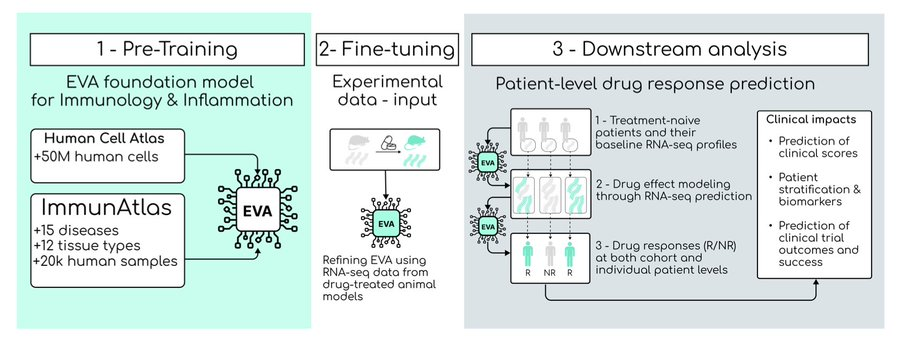
\includegraphics[width=0.95\textwidth]{images/eva_training_pipeline.jpg}
	\captionof{figure}{Pipeline huấn luyện hai giai đoạn của EVA. (1) Pre-training bằng Masked Image Modeling trên dữ liệu web-scale; (2) Fine-tuning bằng học tương phản ngôn ngữ–hình ảnh.}
	\label{fig:eva_pipeline}
\end{center}jpg

---

\textbf{Tóm lại:} EVA không thay đổi kiến trúc Transformer, mà chứng minh rằng với quy mô và cơ chế học tự giám sát đúng đắn, ViT có thể trở thành nền tảng thị giác phổ quát. Đây là minh chứng cho sự chuyển dịch lớn: từ “thiết kế kiến trúc tốt hơn” sang “huấn luyện mô hình lớn hơn, thông minh hơn”.

\subsection{ConvNeXt-V2 (2023): Sự Trở lại của Tích chập}
\label{subsec:convnext_v2}

Sau khi Vision Transformer thống trị giai đoạn 2021–2022, \textbf{ConvNeXt-V2} \cite{Woo2023} từ Meta AI đã mang đến một góc nhìn cân bằng hơn: \textit{CNN không hề lỗi thời, nếu được tái thiết kế và huấn luyện bằng tư duy của thời đại Transformer.}

ConvNeXt-V2 là bước phát triển trực tiếp từ ConvNeXt \cite{Liu2022}, với hai hướng cải tiến chính:
\begin{enumerate}
	\item Tích hợp cơ chế học tự giám sát (self-supervised learning) qua mô hình \textbf{Fully Convolutional Masked Autoencoder (FCMAE)}.
	\item Giới thiệu lớp chuẩn hóa mới \textbf{Global Response Normalization (GRN)}, thay thế LayerNorm, giúp cải thiện tính ổn định và hiệu năng.
\end{enumerate}

---

\subsubsection{Động cơ và Triết lý Thiết kế}
\label{subsubsec:convnext_v2_motivation}

ConvNeXt (2022) đã chứng minh rằng CNN có thể đạt hiệu năng tương đương Transformer nếu được hiện đại hóa theo các nguyên tắc:
- Sử dụng patchify stem.
- Thay BatchNorm bằng LayerNorm.
- Dùng depthwise convolution và GELU.
- Học với các chiến lược huấn luyện hiện đại (AdamW, cosine schedule, augmentation mạnh).

Tuy nhiên, ConvNeXt vẫn phụ thuộc vào huấn luyện có giám sát (supervised learning), trong khi xu hướng hiện đại chuyển dịch sang \textbf{học tự giám sát quy mô lớn} – như MAE, DINOv2 hay EVA. ConvNeXt-V2 ra đời nhằm đưa CNN vào cùng “sân chơi tự giám sát” này.

---

\subsubsection{Fully Convolutional Masked Autoencoder (FCMAE)}
\label{subsubsec:fcmae}

Ý tưởng của FCMAE là \textbf{mở rộng cơ chế Masked Autoencoder (MAE)} — vốn được thiết kế cho ViT — sang một mạng CNN thuần túy.

\begin{itemize}
	\item Trong MAE, ảnh được chia thành các patch, rồi che đi ngẫu nhiên 75\% số patch, và mô hình học cách tái tạo lại chúng thông qua bộ mã hóa–giải mã Transformer.
	\item Với CNN, patch-based masking không phù hợp, do CNN hoạt động trên không gian liên tục và có tính cục bộ cao.
\end{itemize}

Do đó, ConvNeXt-V2 đề xuất \textbf{FCMAE} — một biến thể trong đó:
\begin{enumerate}
	\item Masking được thực hiện trực tiếp trên bản đồ đặc trưng (feature map) thay vì patch.
	\item Encoder là CNN thuần (ConvNeXt), còn decoder là một mạng nhỏ gọn cũng thuần CNN.
	\item Loss được tính theo không gian latent, giúp mô hình học biểu diễn trừu tượng thay vì tái tạo chi tiết pixel.
\end{enumerate}

\textbf{Kết quả:} FCMAE giúp CNN học được các đặc trưng thị giác tổng quát hơn, gần tương đương các ViT tự giám sát (MAE, DINOv2), nhưng với chi phí huấn luyện và suy luận thấp hơn đáng kể.

---

\subsubsection{Global Response Normalization (GRN)}
\label{subsubsec:grn}

Một điểm yếu của CNN là các kênh đặc trưng (feature channels) thường cạnh tranh không cân bằng — một vài kênh chi phối mạnh, khiến biểu diễn kém đa dạng.  
\textbf{Global Response Normalization (GRN)} được giới thiệu để giải quyết vấn đề này.

Công thức GRN cho đầu ra của feature map $x \in \mathbb{R}^{C \times H \times W}$:
\[
\hat{x}_c = \frac{x_c}{\sqrt{\frac{1}{C} \sum_{i=1}^{C} \|x_i\|_2^2 + \epsilon}}
\]

Khác với LayerNorm (chuẩn hóa theo từng vị trí không gian), GRN chuẩn hóa toàn bộ kênh đặc trưng theo \textbf{mức năng lượng toàn cục (global response)}.  
Kết quả là:
\begin{itemize}
	\item Các kênh đặc trưng duy trì cân bằng hơn.
	\item Mạng có khả năng biểu diễn ngữ nghĩa toàn cục tốt hơn, gần giống Transformer.
	\item Huấn luyện ổn định và nhanh hơn, đặc biệt trong pre-training tự giám sát.
\end{itemize}

---

\subsubsection{Hiệu Năng và Thực Nghiệm}
\label{subsubsec:convnext_v2_results}

ConvNeXt-V2 được pre-train bằng FCMAE trên tập dữ liệu ImageNet-22K và fine-tune trên ImageNet-1K, COCO và ADE20K.  
Một số kết quả tiêu biểu:
\begin{itemize}
	\item \textbf{ImageNet-1K:} ConvNeXt-V2-L đạt 88.6\% Top-1 accuracy, tương đương SwinV2-L và ViT-L, vượt ConvNeXt gốc +1.2\%.
	\item \textbf{COCO Detection:} mAP 55.5, vượt ViTDet cùng kích thước.
	\item \textbf{ADE20K Segmentation:} mIoU 58.3, đạt state-of-the-art trong nhóm CNN.
\end{itemize}

Ngoài độ chính xác, ConvNeXt-V2 còn:
\begin{itemize}
	\item Suy luận nhanh hơn ViT cùng quy mô \textbf{30–40\%}.
	\item Tương thích tốt hơn với GPU và phần cứng edge (do chỉ dùng convolution).
	\item Dễ dàng fine-tune cho nhiều nhiệm vụ thị giác khác nhau.
\end{itemize}

\begin{center}
	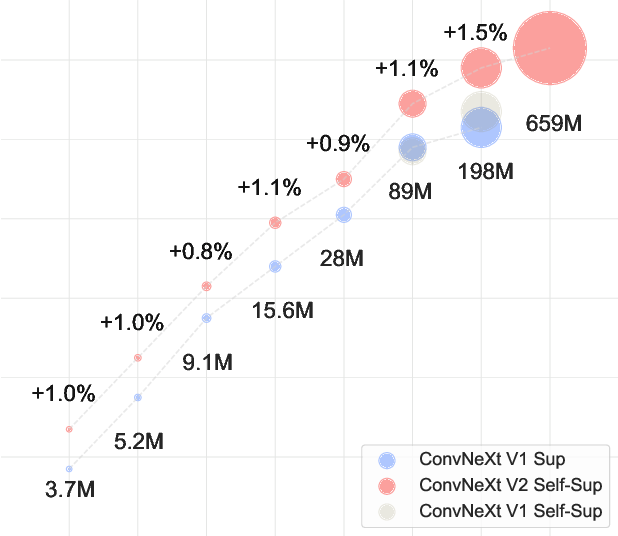
\includegraphics[width=0.9\textwidth]{images/convnext_v2_vs_vit.png}
	\captionof{figure}{So sánh hiệu năng và tốc độ suy luận giữa ConvNeXt-V2 và các Vision Transformer (như ViT, Swin). ConvNeXt-V2 thường nằm trên đường biên Pareto, cho thấy sự cân bằng xuất sắc giữa độ chính xác và hiệu quả.}
	\label{fig:convnext_v2_comparison}
\end{center}

---

\subsubsection{Ý Nghĩa và Vai Trò}
\label{subsubsec:convnext_v2_significance}

ConvNeXt-V2 là minh chứng cho sự “phục hưng” của CNN:
\begin{itemize}
	\item Nó cho thấy rằng \textbf{các ý tưởng tự giám sát và chuẩn hóa toàn cục không chỉ thuộc về Transformer}, mà hoàn toàn có thể áp dụng thành công cho CNN.
	\item FCMAE biến CNN thành một “autoencoder trừu tượng”, mở đường cho các mô hình nền tảng dựa trên tích chập.
	\item GRN giúp CNN thu hẹp khoảng cách giữa cục bộ (local) và toàn cục (global) – yếu tố mà Transformer vốn vượt trội.
\end{itemize}

Với ConvNeXt-V2, ranh giới giữa CNN và Transformer trở nên mờ nhạt hơn bao giờ hết. Thay vì “CNN vs. Transformer”, nghiên cứu thị giác máy tính hiện đại hướng đến một kỷ nguyên mới: \textbf{hợp nhất tư duy giữa hai thế giới — mô hình tích chập hiện đại hóa và mô hình tự chú ý hiệu quả.}

\subsection{InternImage (2023): Sức mạnh của Tích chập Biến dạng và Attention}
\label{subsec:internimage}

\textbf{InternImage} \cite{Wang2023}, được phát triển bởi Shanghai AI Lab, là một trong những nỗ lực tiên phong nhằm phá vỡ ranh giới giữa tích chập (convolution) và cơ chế tự chú ý (attention).  
Thay vì chọn một bên, InternImage \textbf{dung hòa cả hai}, xây dựng một mạng tích chập có khả năng \textit{tự điều chỉnh không gian lấy mẫu} tương tự như self-attention — đưa CNN tiến gần hơn đến khả năng thích ứng ngữ cảnh của Transformer.

---

\subsubsection{Động cơ: Hạn chế của Tích chập Cố định}
\label{subsubsec:internimage_motivation}

Các kernel tích chập truyền thống ($3 \times 3$, $7 \times 7$) lấy mẫu trên một lưới cố định quanh mỗi pixel.  
Mặc dù hiệu quả, nhưng cách lấy mẫu này có hai hạn chế lớn:
\begin{enumerate}
	\item Không thể thích ứng với \textbf{hình dạng, tỷ lệ và vị trí} của vật thể trong ảnh.
	\item Mất khả năng \textbf{nắm bắt ngữ cảnh toàn cục} khi đối tượng thay đổi hình dạng phức tạp.
\end{enumerate}

Ngược lại, self-attention trong Transformer có thể linh hoạt chọn “vị trí quan trọng” ở bất kỳ nơi nào trong ảnh, nhưng chi phí tính toán cao ($O(N^2)$ theo số patch).  
InternImage ra đời để dung hòa hai cực này — \textbf{hiệu quả như tích chập, linh hoạt như attention.}

---

\subsubsection{Deformable Convolution v3 (DCNv3): Nền tảng Của Kiến Trúc}
\label{subsubsec:dcnv3}

Cốt lõi của InternImage là \textbf{DCNv3} — thế hệ thứ ba của Deformable Convolution, mở rộng từ DCNv1 \cite{Dai2017} và DCNv2 \cite{Zhu2019}.  
Trong DCN, thay vì áp dụng kernel $K \times K$ tại các vị trí cố định, ta học thêm hai thành phần:
\begin{itemize}
	\item \textbf{Offset map} $\Delta p$: cho biết mỗi vị trí trong kernel nên “dịch chuyển” đến đâu.
	\item \textbf{Modulation weight} $m$: xác định tầm quan trọng của mỗi vị trí lấy mẫu.
\end{itemize}

Công thức toán học của DCN có dạng:
\[
y(p_0) = \sum_{k=1}^{K} m_k \cdot w_k \cdot x(p_0 + p_k + \Delta p_k)
\]
trong đó:
- $p_0$ là vị trí trung tâm,
- $p_k$ là vị trí gốc của kernel,
- $\Delta p_k$ là offset học được,
- $m_k$ là trọng số điều chế (modulation weight),
- $w_k$ là trọng số tích chập.

DCNv3 mở rộng thêm:
\begin{itemize}
	\item Cơ chế \textbf{offset attention-like}, cho phép offset phụ thuộc không chỉ vào vị trí cục bộ mà còn vào ngữ cảnh rộng.
	\item Thiết kế \textbf{vector hóa hoàn toàn (fully vectorized)}, giúp giảm chi phí bộ nhớ và tăng tốc huấn luyện.
\end{itemize}

Nhờ đó, DCNv3 có thể “nhìn” theo cấu trúc hình học tự nhiên của vật thể, gần tương đương self-attention trong khả năng thích ứng hình dạng, nhưng chỉ với chi phí tuyến tính.

---

\subsubsection{Kiến trúc Block của InternImage}
\label{subsubsec:internimage_block}

Một khối InternImage (InternImage Block) có cấu trúc tương tự như một Transformer block, nhưng thay self-attention bằng DCNv3:
\[
\text{Output} = x + \text{DCNv3}(\text{LN}(x)) + \text{FFN}(\text{LN}(x + \text{DCNv3}(x)))
\]

Cụ thể:
\begin{enumerate}
	\item \textbf{Layer Normalization (LN)} được áp dụng trước mỗi toán tử (pre-norm).
	\item \textbf{DCNv3 module} đóng vai trò như “attention layer”, nắm bắt thông tin không gian linh hoạt.
	\item \textbf{Feed Forward Network (FFN)} gồm hai lớp tuyến tính và hàm kích hoạt GELU, tương tự Transformer.
	\item Kết nối tắt (residual connection) được duy trì xuyên suốt để đảm bảo gradient ổn định.
\end{enumerate}

Nhờ đó, InternImage có thể được huấn luyện và mở rộng như một Transformer, nhưng chạy nhanh hơn đáng kể do thay attention bằng tích chập biến dạng.

\begin{center}
	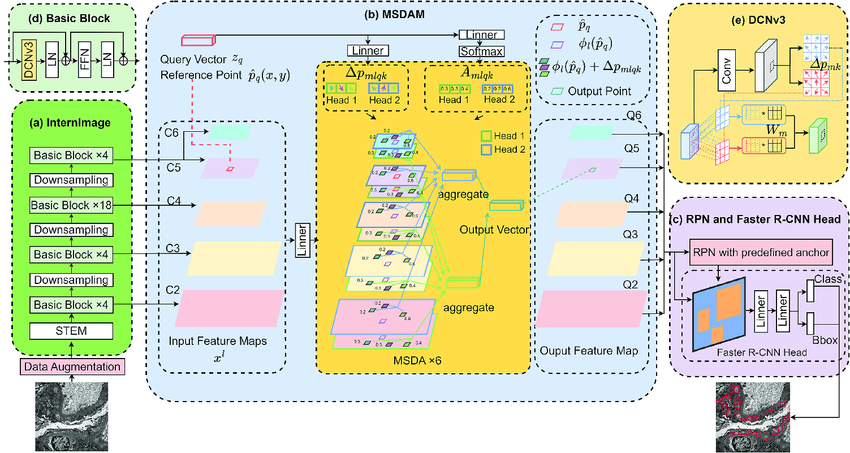
\includegraphics[width=0.9\textwidth]{images/internimage_block.png}
	\captionof{figure}{Cấu trúc khối InternImage. DCNv3 đóng vai trò như một lớp attention cục bộ thích ứng, kết hợp với LayerNorm và FFN tương tự Transformer block.}
	\label{fig:internimage_block}
\end{center}


\subsubsection{Hiệu năng và Ứng dụng}
\label{subsubsec:internimage_results}

InternImage được thiết kế như một \textbf{xương sống (backbone)} cho các mô hình thị giác dày đặc:
\begin{itemize}
	\item \textbf{Phát hiện vật thể (Object Detection):} InternImage-H đạt \textbf{65.4 mAP} trên COCO, vượt Swin-Large và ConvNeXt-L cùng quy mô.
	\item \textbf{Phân đoạn ngữ nghĩa (Segmentation):} Trên ADE20K, đạt \textbf{62.9 mIoU}, thiết lập kỷ lục mới trong nhóm mô hình thuần CNN.
	\item \textbf{Hiệu quả:} Nhờ sử dụng tích chập thay vì self-attention, InternImage có tốc độ suy luận nhanh hơn Transformer tương đương khoảng 30–40\%.
\end{itemize}

Đặc biệt, InternImage đã trở thành nền tảng cho hàng loạt \textbf{mô hình đa phương thức (multimodal foundation models)}:
\begin{itemize}
	\item \textbf{Grounding DINO (2023):} sử dụng InternImage làm backbone để liên kết phát hiện vật thể với hiểu biết ngôn ngữ.
	\item \textbf{InternVL (2023–2024):} kết hợp InternImage với mô hình ngôn ngữ lớn (LLM) để tạo ra hệ thống hiểu biết hình ảnh–văn bản mạnh mẽ, cạnh tranh với CLIP và GPT-4V.
	\item \textbf{InternLM-XComposer:} mở rộng hơn nữa sang lĩnh vực sáng tạo đa phương tiện.
\end{itemize}

---

\subsubsection{Ý Nghĩa và Đóng góp}
\label{subsubsec:internimage_significance}

InternImage đánh dấu một bước ngoặt quan trọng trong tiến hóa của CNN:
\begin{itemize}
	\item Nó chứng minh rằng \textbf{attention không chỉ là cơ chế truy hồi ngữ cảnh toàn cục}, mà bản chất của nó — khả năng “thích ứng không gian” — có thể được mô phỏng hiệu quả bằng \textbf{tích chập biến dạng}.
	\item DCNv3 đưa CNN trở lại trung tâm của cuộc đua foundation models, cạnh tranh sòng phẳng với ViT và Swin.
	\item Với hiệu năng cao, khả năng mở rộng tốt và tích hợp mượt mà trong các pipeline đa phương thức, InternImage được xem là một trong những “backbone của kỷ nguyên foundation”.
\end{itemize}

\begin{mdframed}[style=infobox]
	\textbf{Tóm tắt đóng góp của InternImage:}
	\begin{itemize}
		\item Giới thiệu \textbf{DCNv3} – biến thể mạnh nhất của Deformable Convolution.
		\item Kết hợp thiết kế chuẩn hóa và FFN từ Transformer.
		\item Đạt state-of-the-art trên COCO, ADE20K và nhiều benchmark dày đặc.
		\item Trở thành nền tảng cho các mô hình đa phương thức hàng đầu như Grounding DINO và InternVL.
	\end{itemize}
\end{mdframed}

\subsection{FocalNet (2022): Cơ chế Chú ý Tập trung}
\label{subsec:focalnet}

\textbf{FocalNet} \cite{Yang2022}, một công trình của Microsoft Research, tiếp tục chuỗi nghiên cứu hướng tới việc tối ưu hoá hiệu quả tính toán của các mô hình Vision Transformer.  
Thay vì dựa trên self-attention toàn cục hoặc attention theo cửa sổ (như Swin Transformer), FocalNet giới thiệu một cơ chế mới – \textbf{Focal Modulation} – nhằm mô hình hóa ngữ cảnh theo cách \textit{tập trung và đa cấp độ}, vừa hiệu quả vừa giàu thông tin.

---

\subsubsection{Động cơ: Giới hạn của Self-Attention và Window Attention}
\label{subsubsec:focalnet_motivation}

Cơ chế self-attention truyền thống cho phép mỗi token tương tác với tất cả các token còn lại, mang lại khả năng nắm bắt ngữ cảnh toàn cục mạnh mẽ, nhưng có độ phức tạp tính toán $O(N^2)$ theo số lượng patch.  
Swin Transformer giải quyết bằng cách \textbf{chia ảnh thành các cửa sổ cục bộ}, chỉ tính attention trong phạm vi cửa sổ, giúp giảm độ phức tạp xuống $O(N)$ nhưng đánh đổi khả năng mô hình hóa tầm xa.

\textbf{FocalNet} tìm cách dung hòa hai cực này bằng cách cho phép mỗi token:
\begin{itemize}
	\item tập trung vào các vùng lân cận quan trọng,
	\item đồng thời vẫn tổng hợp được thông tin ngữ cảnh đa cấp độ.
\end{itemize}

---

\subsubsection{Cơ chế Focal Modulation}
\label{subsubsec:focal_modulation}

Focal Modulation là một phương pháp tổng hợp ngữ cảnh mà không cần tính toán attention giữa từng cặp token.  
Nó bao gồm ba bước chính:

\begin{enumerate}
	\item \textbf{Tổng hợp ngữ cảnh đa cấp độ:}  
	Các đặc trưng được gộp (pooled) ở nhiều tỷ lệ không gian khác nhau (ví dụ $1 \times 1$, $3 \times 3$, $5 \times 5$) để thu nhận thông tin ngữ cảnh tầm gần và tầm xa.  
	Quá trình này tương tự như “multi-scale receptive field” trong CNN.
	
	\item \textbf{Kết hợp ngữ cảnh (Context Fusion):}  
	Các ngữ cảnh ở nhiều cấp độ được kết hợp bằng một hàm học được (learnable fusion function), tạo ra một vector \textbf{modulation signal} duy nhất cho mỗi token.
	
	\item \textbf{Điều biến đặc trưng (Feature Modulation):}  
	Ngữ cảnh tổng hợp này được dùng để “điều biến” (modulate) đặc trưng của token trung tâm thông qua phép nhân tuyến tính hoặc phi tuyến:
	\[
	\tilde{x}_i = f(x_i, c_i) = \sigma(W_c \cdot c_i) \odot x_i
	\]
	trong đó $x_i$ là đặc trưng ban đầu, $c_i$ là vector ngữ cảnh, và $\sigma$ là hàm kích hoạt.
\end{enumerate}

Như vậy, thay vì tính attention ma trận giữa mọi cặp token, FocalNet chỉ tính toán một số lượng nhỏ các phép gộp cục bộ và điều biến tuyến tính, giúp giảm đáng kể chi phí tính toán mà vẫn giữ khả năng nắm bắt ngữ cảnh toàn cục.

\begin{center}
	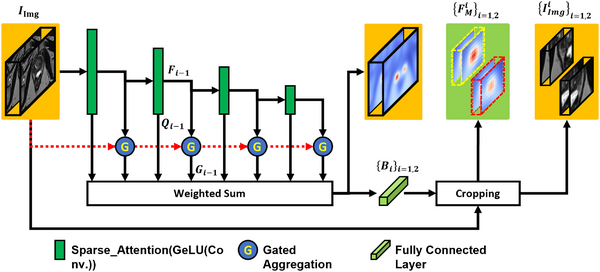
\includegraphics[width=0.9\textwidth]{images/focal_modulation.png}
	\captionof{figure}{Minh họa cơ chế Focal Modulation. Mỗi token tổng hợp ngữ cảnh từ các vùng lân cận ở nhiều cấp độ, sau đó sử dụng tín hiệu ngữ cảnh để điều biến đặc trưng của chính nó.}
	\label{fig:focal_modulation}
\end{center}

---

\subsubsection{Hiệu năng và So sánh}
\label{subsubsec:focalnet_results}

Nhờ thiết kế này, FocalNet đạt hiệu năng ấn tượng trên nhiều tác vụ thị giác mà vẫn duy trì hiệu quả cao:

\begin{itemize}
	\item \textbf{Phân loại ảnh (ImageNet-1K):}  
	FocalNet-Large đạt 85.3\% Top-1 accuracy, tương đương Swin-Large nhưng với ít phép tính FLOPs hơn khoảng 25\%.
	\item \textbf{Phát hiện vật thể (COCO):}  
	Khi dùng làm backbone cho Mask R-CNN, FocalNet tăng khoảng 1.2 mAP so với Swin với cùng cấu hình.
	\item \textbf{Phân đoạn ngữ nghĩa (ADE20K):}  
	FocalNet đạt 52.5 mIoU, vượt ConvNeXt và ngang Swin-L.
\end{itemize}

Đặc biệt, nhờ loại bỏ self-attention ma trận, FocalNet có thể mở rộng lên độ phân giải cao hơn mà không tăng mạnh chi phí bộ nhớ, giúp nó phù hợp với các ứng dụng thực tế như segmentation hay video understanding.

---

\subsubsection{Ý Nghĩa và Ảnh hưởng}
\label{subsubsec:focalnet_significance}

FocalNet thể hiện một hướng tư duy mới trong thiết kế Transformer cho thị giác:
\begin{itemize}
	\item Nó chứng minh rằng khả năng “tổng hợp ngữ cảnh” của self-attention có thể được tái tạo bằng cơ chế điều biến đa cấp độ, không cần phép nhân ma trận tốn kém.
	\item Cơ chế Focal Modulation đóng vai trò như một cầu nối giữa attention và convolution – sử dụng pooling đa tỷ lệ (như CNN) nhưng kết hợp phi tuyến theo ngữ cảnh (như Transformer).
	\item Nhờ tính hiệu quả, FocalNet được dùng làm backbone trong nhiều mô hình đa phương thức sau này (ví dụ EVA-CLIP và BEiT-3), giúp giảm đáng kể chi phí huấn luyện mà vẫn giữ hiệu năng cao.
\end{itemize}

\begin{mdframed}[style=infobox]
	\textbf{Tóm tắt đóng góp của FocalNet:}
	\begin{itemize}
		\item Đề xuất \textbf{Focal Modulation} – cơ chế tổng hợp ngữ cảnh hiệu quả thay thế self-attention.  
		\item Giảm đáng kể chi phí tính toán mà vẫn duy trì khả năng mô hình hóa toàn cục.  
		\item Đạt hiệu năng SOTA trên ImageNet, COCO, ADE20K.  
		\item Đặt nền móng cho hướng nghiên cứu attention hiệu quả (efficient attention) trong các foundation models sau này.
	\end{itemize}
\end{mdframed}

\subsection{Xu hướng Định hình Tương lai (2025 và xa hơn)}
\label{subsec:future_trends_2025}
Các kiến trúc SOTA này không phải là những nỗ lực riêng lẻ, mà là những biểu hiện của các xu hướng lớn hơn đang định hình tương lai của thị giác máy tính:
\begin{description}
	\item[Hướng tới các Mô hình Thống nhất (Unified Models):] Mục tiêu cuối cùng là xây dựng các mô hình nền tảng duy nhất, có thể được "prompt" để giải quyết nhiều tác vụ thị giác khác nhau (phân loại, phát hiện, phân đoạn, tạo chú thích, trả lời câu hỏi,...) mà không cần phải huấn luyện lại các mô hình chuyên biệt.
	\item[Học Tự giám sát ở Quy mô Cực lớn:] Các phương pháp như Masked Image Modeling (MIM) và học tương phản sẽ tiếp tục là động lực chính để huấn luyện các mô hình nền tảng trên dữ liệu web, giúp chúng học được một sự "thấu hiểu" sâu sắc về thế giới thị giác.
	\item[Hợp nhất Thị giác và Ngôn ngữ:] Ranh giới giữa hai lĩnh vực sẽ ngày càng mờ đi. Các Mô hình Ngôn ngữ Lớn Đa phương thức (LMMs), có khả năng "nhìn" và "lý luận" về hình ảnh, sẽ trở thành trung tâm của nhiều ứng dụng AI thế hệ mới.
	\item[Sự hội tụ của CNN và Transformer:] Cuộc tranh luận về kiến trúc sẽ không còn là "ai thắng ai", mà là "kết hợp như thế nào". Các ý tưởng tốt nhất từ cả hai thế giới sẽ tiếp tục được hòa trộn, tạo ra các kiến trúc lai ngày càng mạnh mẽ và hiệu quả.
\end{description}
Giai đoạn 2024–2025 chứng kiến một sự hợp nhất của các xu hướng, nơi các mô hình không chỉ mạnh hơn về mặt học thuật mà còn linh hoạt và tổng quát hơn cho các ứng dụng thực tế. EVA, ConvNeXt-V2, InternImage và FocalNet là những đại diện tiên phong cho thế hệ mô hình thị giác mới này, hướng tới một tương lai nơi một mô hình duy nhất có thể đi từ pixel đến nhận thức một cách toàn diện.

\section*{Tài liệu tham khảo}
\begin{itemize}
	\item[1] Fang, Y., Wang, W., Xie, Z., Chen, Z., Wang, X., Qiao, Y., ... \& Cao, Y. (2023). Eva: Exploring the limits of masked visual representation learning at scale. In \textit{Proceedings of the IEEE/CVF Conference on Computer Vision and Pattern Recognition (CVPR)}. (Paper giới thiệu EVA-01).
	\item[2] Sun, Q., Fang, Y., Wang, W., Yuan, H., Chen, Z., Wang, X., ... \& Cao, Y. (2023). Eva-02: A visual representation for neon genesis. \textit{arXiv preprint arXiv:2303.11331}. (Paper giới thiệu EVA-02 và các cải tiến).
	\item[3] Woo, S., Debnath, S., Hu, R., Chen, X., Liu, Z., Lapedriza, A., \& Dollar, P. (2023). Convnext v2: Co-designing and scaling convnets with masked autoencoders. In \textit{Proceedings of the IEEE/CVF Conference on Computer Vision and Pattern Recognition (CVPR)}. (Paper gốc giới thiệu ConvNeXt-V2).
	\item[4] Wang, W., Zhou, D., Li, Z., Wang, W., Wang, X., Liu, Z., ... \& Qiao, Y. (2023). Internimage: Exploring large-scale vision foundation models with deformable convolutions. In \textit{Proceedings of the IEEE/CVF Conference on Computer Vision and Pattern Recognition (CVPR)}. (Paper gốc giới thiệu InternImage).
	\item[5] Yang, J., Li, C., Zhang, P., Dai, X., Xiao, B., Yuan, L., \& Gao, J. (2022). Focal modulation networks. In \textit{Advances in Neural Information Processing Systems (NeurIPS)}. (Paper gốc giới thiệu FocalNet, xuất bản cuối 2022 nhưng ảnh hưởng lớn trong 2023-2024).
	\item[6] He, K., Chen, X., Xie, S., Li, Y., Dollár, P., \& Girshick, R. (2022). Masked autoencoders are scalable vision learners. In \textit{Proceedings of the IEEE/CVF conference on computer vision and pattern recognition (CVPR)}. (Paper giới thiệu MAE, phương pháp self-supervised nền tảng cho nhiều mô hình SOTA).
\end{itemize}